\documentclass[10pt]{article}
\usepackage{grafematik}

\title{Malayalam Orthographic Reforms: \\Impact on Language and Popular Culture}

\author{Kavya Manohar \\
\small{Swathanthra Malayalam Computing\footnote{\url{https://smc.org.in}}} \\
 {\small {\tt sakhi.kavya@gmail.com}} \\
 \and
 Santhosh Thottingal \\
 \small{Swathanthra Malayalam Computing} \\
 {\small {\tt santhosh.thottingal@gmail.com}}}

\begin{document}

\maketitle

\begin{abstract}

Malayalam is a language spoken in India, predominantly in the state of Kerala with about 38 million native speakers. The Malayalam script evolved from Brahmi through Grantha alphabet and Vattezhuthu writing systems. The script orthography has acquired its uniqueness with its complex shaped graphemes formed by the combination of consonant sequences and signed vowel forms. The number of unique graphemes in this system exceeds twelve hundred. The orthographic styles were constantly evolving. In 1971 there was a Governmental intervention in the orthograhy, to reduce its complexity to address the difficulties in typesetting and printing. This paper is an attempt to explore the impact of this orthographic reforms on various aspects of script usage including popular culture, media, textbooks, graffiti and handwriting. We will also analyse the impact of Unicode and the advancement in digital typography on the orthographic diversity of Malayalam script.

\end{abstract}
 \textbf{Keywords:} Malayalam Script, Orthography Reforms, Unicode, Graphemes, Media and Communication, Digital Typography

\section{Introduction}

\paragraph{}
With 38 million native speakers Malayalam is the official language of Kerala, in southern India. Malayalam used to be written in Vattezhuthu, the then script for Tamil, another south Indian language. The modern Malayalam script evolved from Grantha alphabet which was a script for Sanskrit. Both Vattezhuthu and Grantha has its roots in the Brahmi script\footnote{Malayalam Script in English Wikipedia: \url{https://en.wikipedia.org/wiki/Malayalam_script}}. Unicode has encoded 18 vowels and 37 consonants as of today, some of them are archaic.  The Figure \ref{unicode} illustrates the malayalam codeblock as per Unicode 10.0\footnote{Malayalam Unicode block: \url{https://unicode.org/charts/PDF/U0D00.pdf}}. 


\begin{figure}[h!]
	\centering
	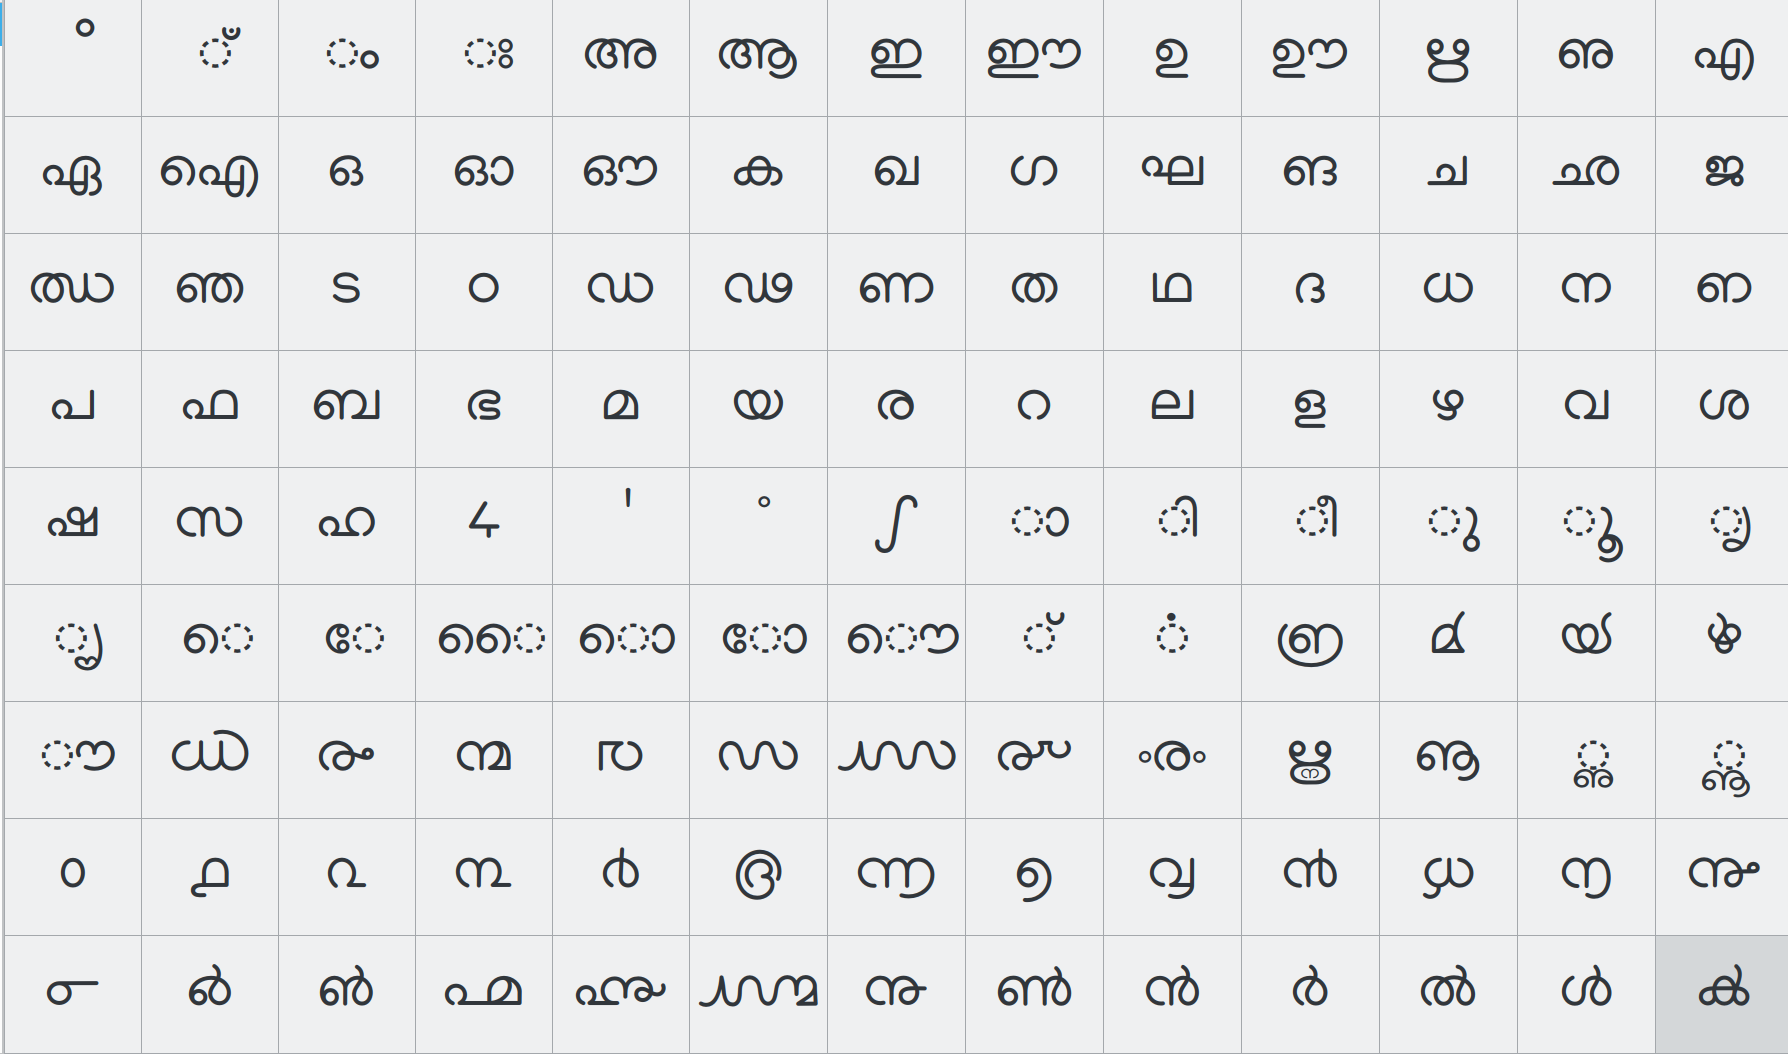
\includegraphics[scale=0.2]{images/unicodeml.png}
	\caption{Unicode 10.0 Malayalam Codeblock}
	\label{unicode}
\end{figure} 


\paragraph{}
Malayalam script is abugida, or alphasyllabary. That is, consonant–vowel sequences are written as a unit: each unit is based on a consonant or conjunct letter, and vowel notation is secondary. Vowels have independent existence, but only at word beginnings. This is the common characterestic of Brahmic family of scripts from South and Southeast Asia.


\begin{figure}[h!]
	\centering
	
\includegraphics[scale=0.4]{images/malayalamExamples.png}
	\caption{Few samples of graphemes in Malayalam}
	\label{malayalamsamples}
\end{figure} 


\paragraph{}
The script has acquired its uniqueness with it's complex shaped ligatures formed by the consonants and conjuncts with signed vowel forms. Conjuncts are formed by a sequence of two more consonants. The conjunct grapheme usually has a shape smoothly blend from the constituent consonants. Figure \ref{malayalamsamples} illustrates some samples.


\section{Script in Early Printing Era}

\paragraph{}
The shapes of conjuncts, relative positioning of signs and their sizes have changed over time to match the needs of writing methods. Stylus on dry palm leaves gave limited flexibility and the graphemes were rarely perfect rounds. But pen on paper made it more curvy. See Figure \ref{palmleaves}.

\begin{figure}[h!]
	\centering
	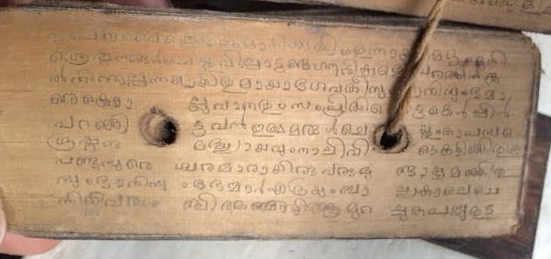
\includegraphics[width=0.8\textwidth]{images/manuscipt.png}
	\caption{Manuscript on palm leaves}
	\label{palmleaves}
\end{figure} 

\paragraph{}
The first ever book in Malayalam script was printed in Rome, in 1772. Printing in Malayalam started natively during 1820s\cite{babucherian}. When printing technology started getting popular there was a requirement to cast movable types in huge numbers. Even though the basic characters were less than hundred, the orthographic style demanded separate types for conjuncts, and their signed vowel forms. Apart from vowels, some consonants too have signed notations, further increasing the number of types needed in the foundry. 

\begin{figure}[h!]
	\centering
	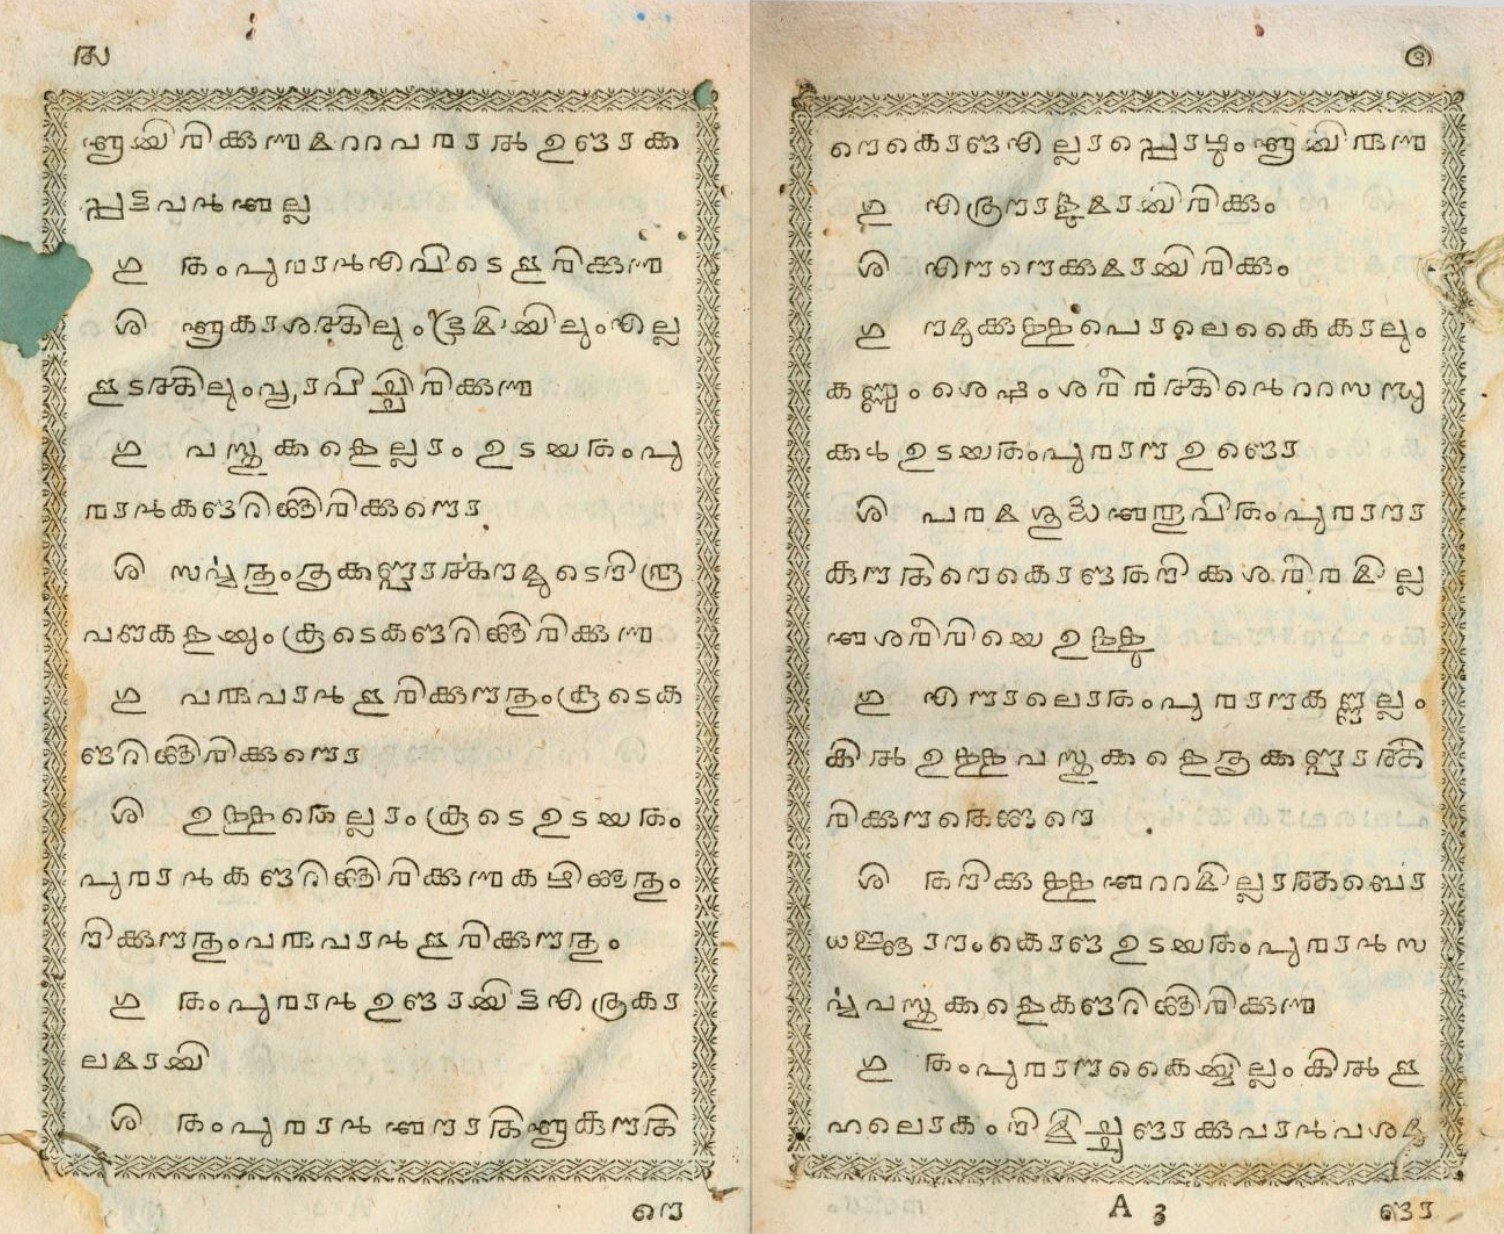
\includegraphics[width=\textwidth]{images/samkshepavedartham1772.png}
	\caption{Samkshepavedartham - 1772}
	\label{Samkshepam}
\end{figure} 


\paragraph{}
The first printed book in Malayalam using movable types, {\manjari സംക്ഷെപവെദാർത്ഥം} (Samkshepavedartham) in 1772 had more than thousand unique types\cite{babucherian}. The manual labour on typesetting and lay outing were high for the same reason. Figure \ref{Samkshepam} shows pages from the catechism book Samkshepavedartham. The script is mostly rectangular. The types were made and printing was done in Rome. 

\paragraph{}
The first native type casting and printing was done by Benchamin Bailey, an Anglican missionary in 1829\cite{babucherian}.  His contributions as a typographer made the curvy style of the Malyalam orthography popular\cite{gupthannair}. Figure \ref{newtestament}, shows pages from The New Testament printed using the types designed by Benchamin Bailey, imprinted in 1829\cite{babucherian}. The script continued to evolve by separating some vowel sign types ({\manjari{  ി, ീ } }) from the consonant/conjunct grapheme. Still the richness of conjuncts and their signed forms were largely retained. It can be seen from Figure \ref{Sabdatharavali}. 

\begin{figure}[H]

\begin{subfigure}{0.75\textwidth}
 \centering
 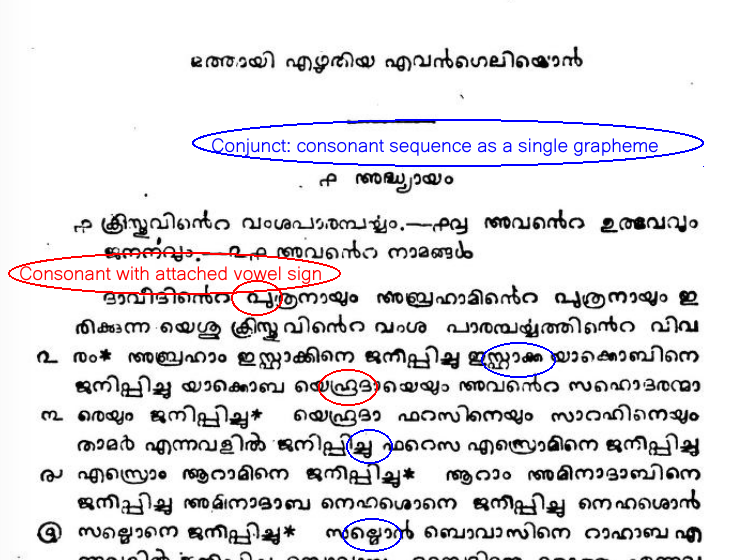
\includegraphics[width=\linewidth]{images/newtestament1829.png}
 \caption{New Testament - 1829}
 \label{newtestament}
\end{subfigure}
\\ \\
\begin{subfigure}{0.75\textwidth}
 \centering
 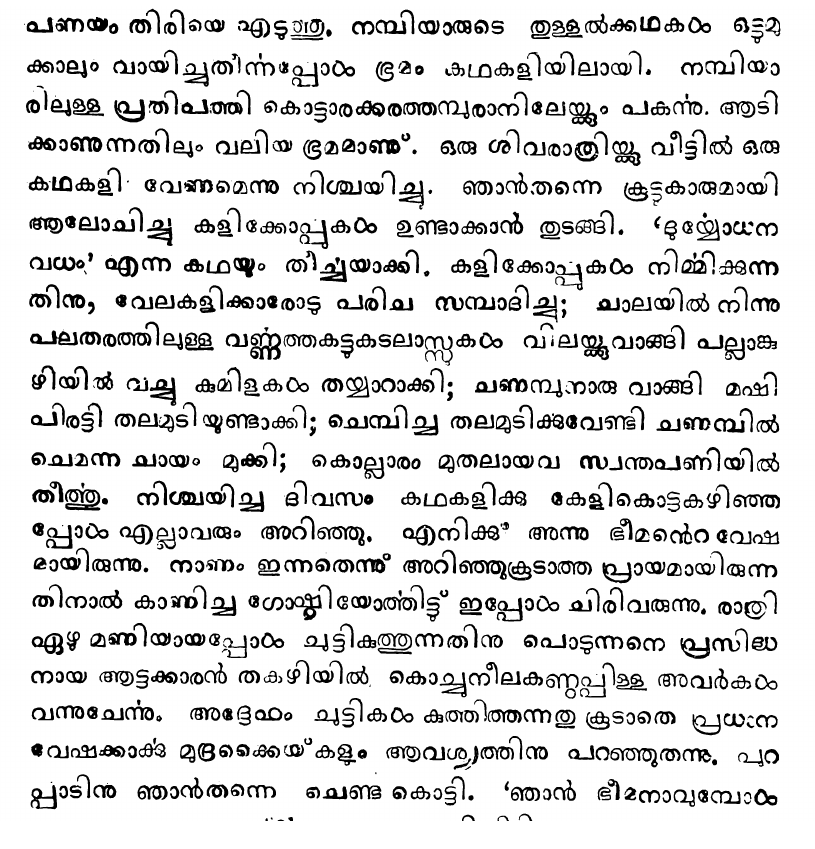
\includegraphics[width=\linewidth]{images/1930-Sabdatharavali.png}
 \caption{Sabdatharavali - 1930 }
 \label{Sabdatharavali}
\end{subfigure}
\caption{Samples of print documents. Complex graphemes formed by consonant sequences and signed conjuncts can be seen.}
\end{figure}


\section{Script Reformation}

\paragraph{}
Typewriters became very popular around 1960s in Kerala. These typewriters followed the same design of English typewriters with the keys repurposed for Malayalam. Obvioulsly the keys were not enough to support all complex ligatures. The end result was Malayalam with all ligatures split up. It was a painful experience for reading and did not do any justice to the beauty of script as we can observe from Figure \ref{typewriter}.

\begin{figure}[h!]
	\centering
	\begin{subfigure}{.7\textwidth}
		\centering
		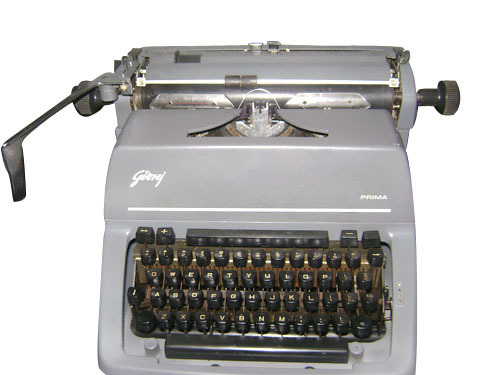
\includegraphics[width=\linewidth, height=5cm]{images/godrej-typewriter.jpg}
		\caption{Godrej typewriter}
		\label{godrej}
	\end{subfigure}%
	\\
	\begin{subfigure}{\textwidth}
		\centering
		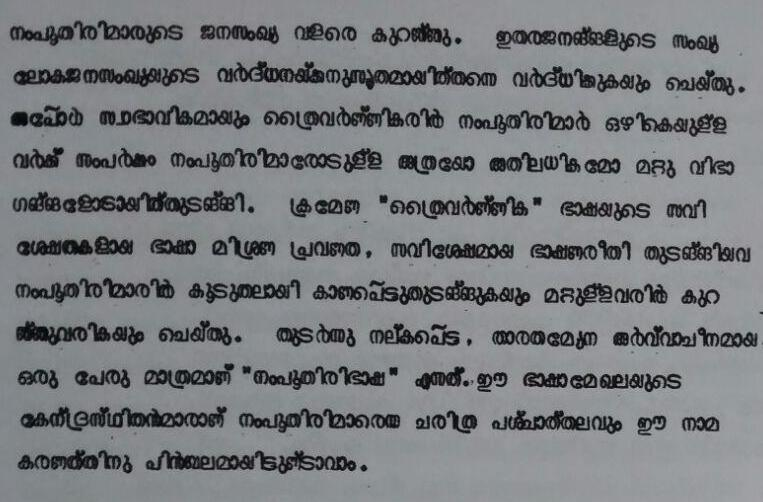
\includegraphics[width=\linewidth,height=6.5cm]{images/typewritertext4.jpg}
		\caption{Malayalam script typed by a typewriter}
		\label{typewritertext}
	\end{subfigure}
	\caption{A typewriter and a sample of Malayalam document prepared using typewriter No complex graphemes are used. Consonant sequences remain separated with \textit{virama} in between}
	\label{typewriter}
\end{figure}

\paragraph{}
To solve this either the typewriter or language had to be redesigned. There were demanads from newspaper and publishing industries to reduce the script complexity so that Malayalam is better suited for typewriters and priting. Based on this, in 1967 Kerala government appointed a committee to study script reformation. The committee submitted their report and in 1971 Kerala governmet published an order to reduce the complexity of the script\cite{1971go}.

\paragraph{}
The order was to discard the usage of complex conjuncts and to detach the vowel notations from the consonants and conjuncts. Being a forced intervention, this was a major event to be marked in the history of orthographic evolution. 

\paragraph{}
The script variant of Malayalam that came into existance after the reformation order will henceforth be refered as \textit{reformed orthography}. To the understand the effects of the order, we nee to examine the the characteristics of graphemes in \textit{traditional orthography} of Malayalam script.

\subsection{Nature of script}

\begin{itemize}
	\item
	Vowels and consonants are the basic building blocks of Malayalam script.
	\item
	Vowels have stand alone existence in their pure form. Vowels in Malayalam are {\manjari അ, ഇ, എ }etc.
	\item
	Vowels also appear as signed form modifying a consonant sound. Vowel signs have no existance without a consonant. Vowel signs in Malayalam are {\manjari  ി, ീ, െ, ൊ }etc.
	\item Consonants in Malayalam always have the inherent vowel /a/, also known as \textit{schwa} present in them. Consonants in Malayalam are {\manjari ക, ത, ഗ, ദ, ധ }etc.
	\item
	Any other vowels sound, other than /a/  associated with a consonant is written as a signed form of the consonant. The vowel signs can  appear left, right or both with respect to a consonant. Some signs modify the shape of base grapheme. Examples for consonants with vowel signs:  {\manjari കി, ഗു, ധെ, ദൊ} 
	\item 
	The removal of inherent /a/ in a consonant is marked in the script by a special character \textit{virama}. Example for consonant with virama (് ) sign: {\manjari ക് }. Virama after a consonant not only removes inherent /a/ but also indicate no vowel sound follows it. 
	\item
	A conjunct is formed by  a sequence of consonants connected using Virama. Example: {\manjari ക+്+ത -> ക്ത , ഗ+്+ദ ->ഗ്ദ }. A conjunct can again connect to another consonant using Virama and form a longer conjunct. {\manjari ഗ്ദ+്+ധ ->ഗ്ദ്ധ }
	\item	
	Every conjunct can be modified by a vowel sign forming a new ligature. 
	{\manjari ഗ്ദ+്+ധ +ു ->ഗ്ദ്ധു }
	\item
	Some consonants involved in the formation of conjuncts have signed forms. eg:{\manjari ്‌ര, ്‌ല, ്‌യ, ്‌വ, ര് . ക+്‌ര -> ക്ര, ക+്‌ല ->ക്ല , ക+്‌യ -> ക്യ, ക്+്‌വ -> ക്വ, ര്+ക-> ൎക}
	\item 
	Certain consonants have a unique grapheme representation in their pure form named \textit{chillu}. {\manjari ൿ, ൾ, ൺ, ൻ, ൽ, ർ }
\end{itemize}


\begin{figure}[h!]
	\centering
	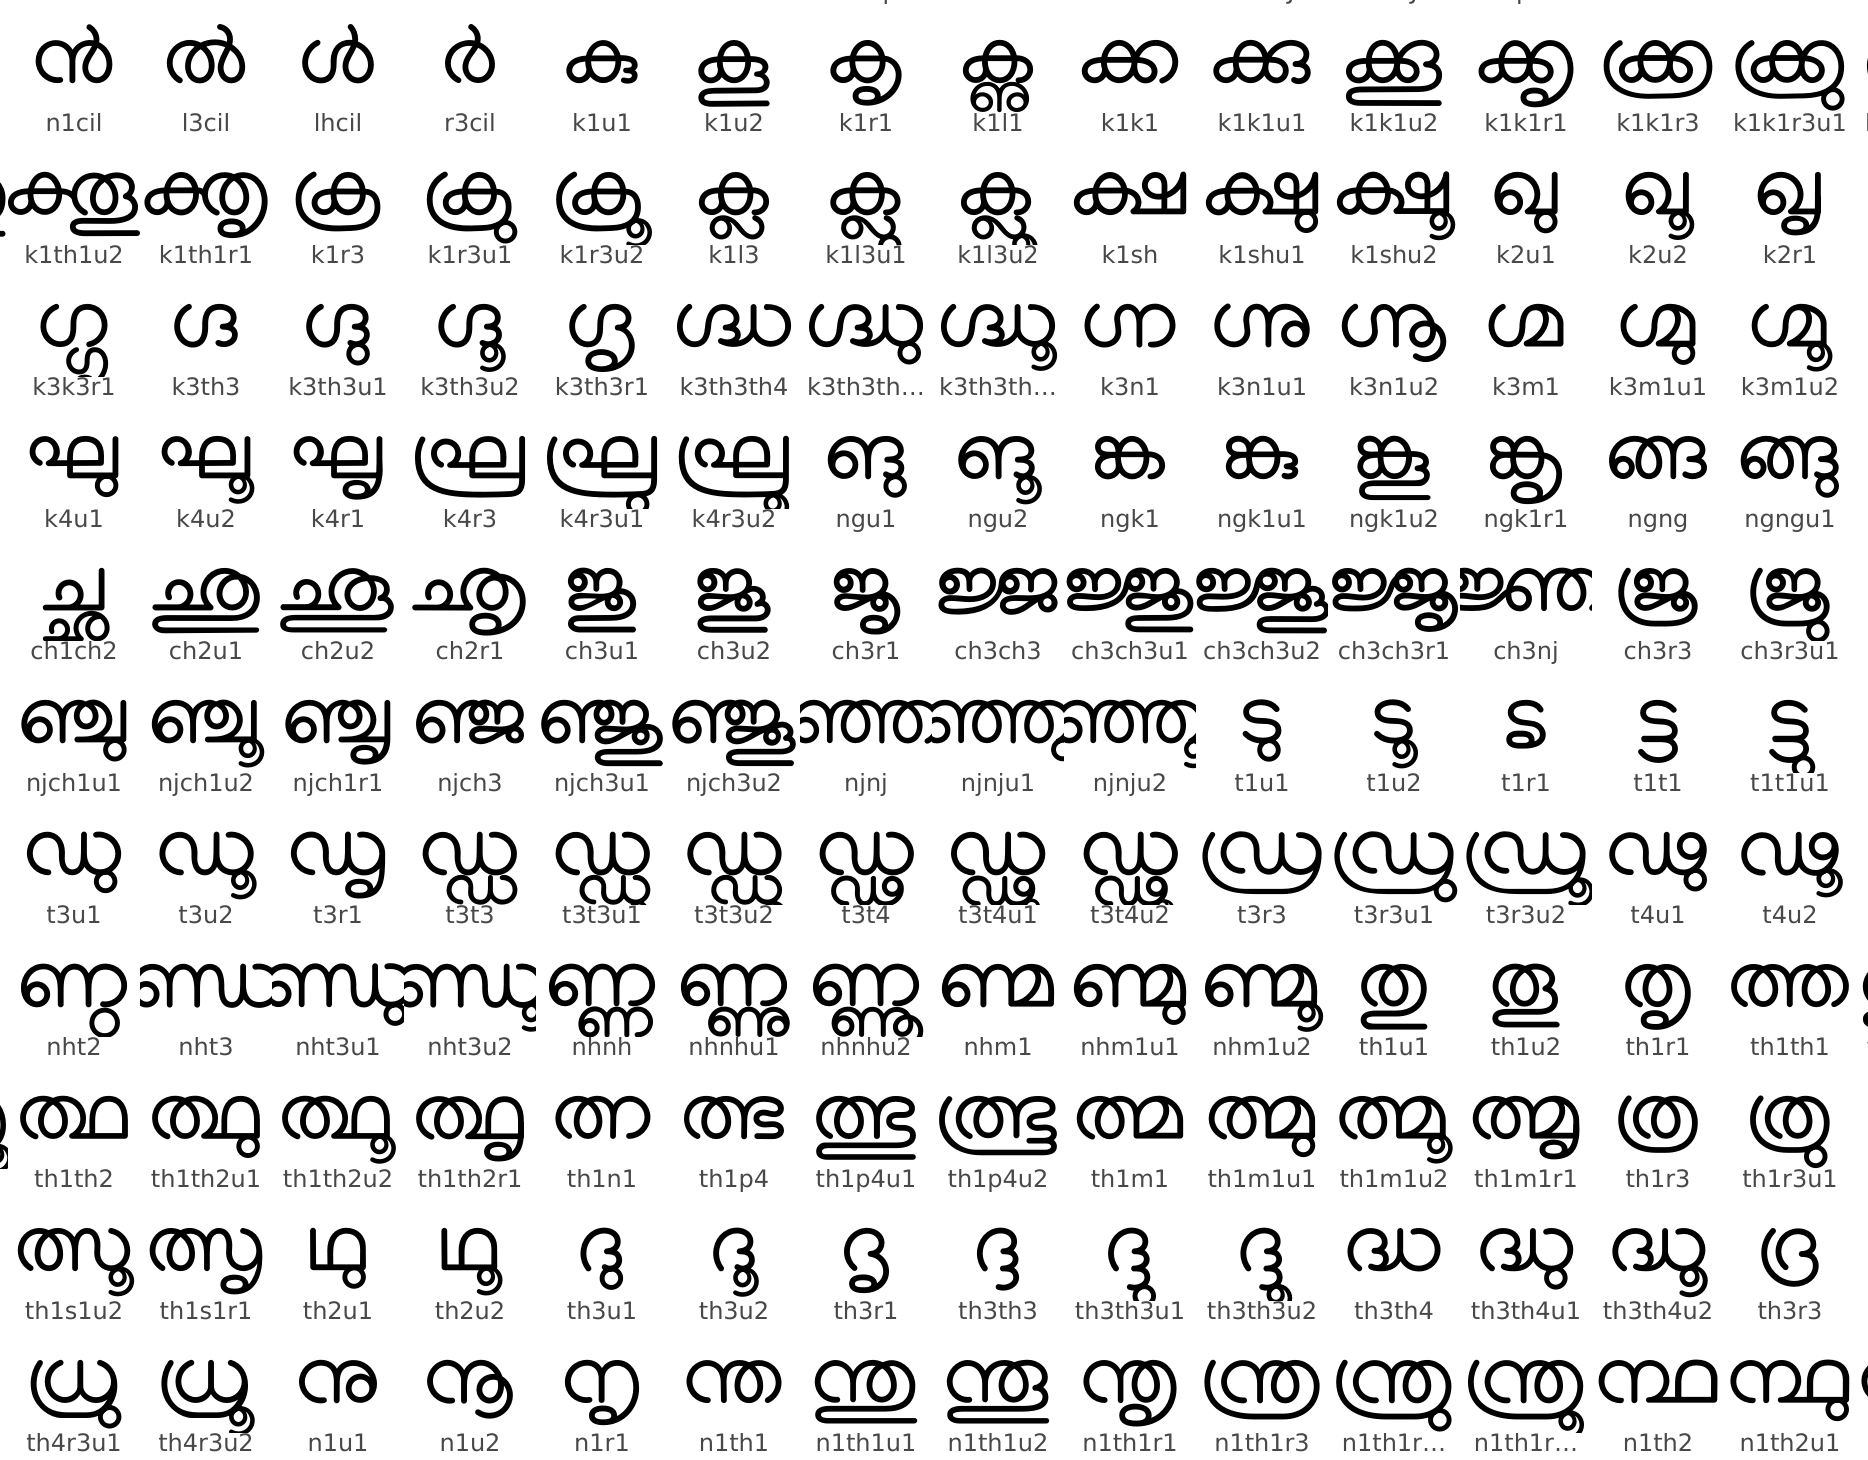
\includegraphics[width=0.8\textwidth]{images/complexgraphemes.png}
	\caption{Set of complex graphemes in Malayalam script}
	\label{complexgrapheme}
\end{figure}


\begin{figure}[h!]
	\centering
	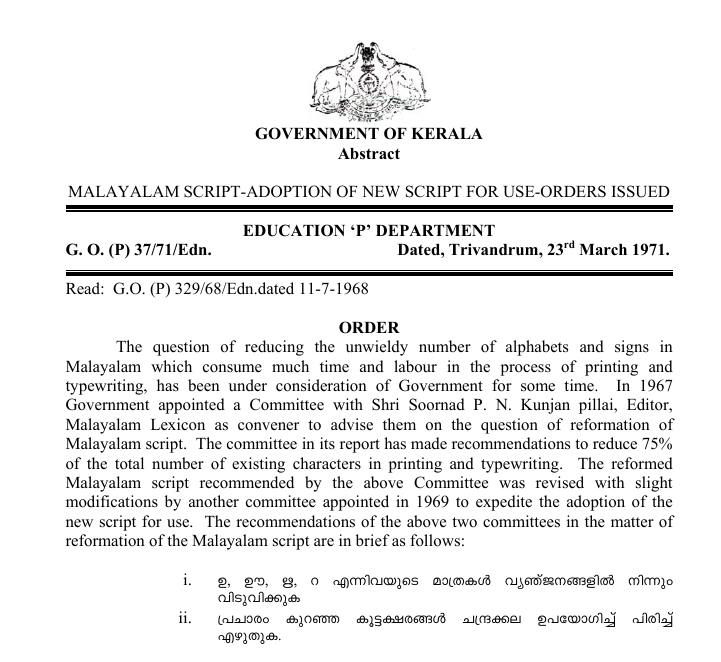
\includegraphics[width=0.8\textwidth]{images/1971-gov-script-reformation-order.png}
	\caption{The Government Order on Malayalam Script Reform in 1971}
	\label{go1971}
\end{figure}

Figure \ref{go1971} shows the front page of government order proposing the new orthography style. The proposal aimed at reducing the grapheme usage in Malayalam by 75\%. The major proposals in the order are following: \cite{1971go}


\begin{table}
	\centering
	
	\begin{tabular}{|c|c|c|c}
		\hline
		Character Sequence & Traditional Orthography & Reformed Orthography \\ \hline \hline
		{\manjari ക, ാ} & {\manjari കാ} & {\raghu കാ} \\
		\hline
		{\manjari ദ,െ} & {\manjari ദെ} & {\raghu ദെ}  \\
		\hline
		{\manjari ക,്, യ} & {\manjari ക്യ} & {\raghu ക്യ} \\
		\hline
		{\manjari ക,്, ക} & {\manjari ക്ക} & {\raghu ക്ക} \\
		\hline
		{\manjari ക ,ു} & {\manjari കു} & {\raghu കു} \\
		\hline
		{\manjari ഗ,ു} & {\manjari ഗു} & {\raghu ഗു} \\
		\hline
		{\manjari ഗ,്, ദ} & {\manjari ഗ്ദ} & {\raghu ഗ്ദ} \\
		\hline
		{\manjari ഗ,്, ദ,ു} & {\manjari ഗ്ദു} & {\raghu ഗ്ദു} \\
		\hline
		{\manjari ഷ,്, ട} & {\manjari ഷ്ട} & {\raghu ഷ്ട} \\	
		\hline
		{\manjari ക,്, ര} & {\manjari ക്ര} & {\raghu ക്ര} \\
		\hline
		{\manjari സ,്, ത,്, ര} & {\manjari സ്ത്ര} & {\raghu സ്ത്ര} \\
		\hline
		{\manjari ക,്, ര,ു} & {\manjari ക്രു} & {\raghu ക്രു} \\
		\hline
		
	\end{tabular}
	\caption{Illustrating traditional and reformed orthography differences}
	\label{orthographycomparison}
\end{table}

\begin{itemize}
\item
Detach the signs of vowels {\manjari ഉ, ഊ and ഋ } from the base grapheme.\\
{\manjari കു } -> {\raghu കു } ,
{\manjari കൂ } -> {\raghu കൂ } ,
{\manjari കൃ } -> {\raghu കൃ } .
\item 
Detach the consonat sign {\manjari  ്ര } from the base grapheme \\
{\manjari ക്ര  } -> {\raghu ക്ര  } 
\item
Discard the usage of {\manjari ര് } in the consonant sequence in signed form as dot reph {\manjari ൎ }. Instead use the alternate form of {\manjari ർ }. {\manjari അൎക്കൻ } -> {\manjari അർക്കൻ }

\item
Discard the use of rare conjuncts by splitting them down into constituent consonant sequence separated by the virama sign. Those retained are: {\manjari ക്ക, ങ്ക, ങ്ങ, ച്ച, ഞ്ച, ഞ്ഞ, ട്ട, ണ്ട, ണ്ണ, ത്ത, ന്ത, ന്ന, പ്പ, മ്പ, മ്മ, യ്യ, ല്ല, വ്വ }. Others are split down as: {\manjari ഗ്ദ } -> {\raghu ഗ്ദ }. 

\item
The signed form of consonants are to be separated from the base grapheme as in {\raghu ക്യ, ക്വ, ക്ര }.

\item
The signed \textit{below base modifiers} of {\manjari  ്‌ല  (്ല )  } may be retained as such {\manjari പ്ല } or split using \textit{virama} sign as {\manjari  പ്‌ല }.

\end{itemize}

\paragraph{}
Table \ref{orthographycomparison} compares the graphemes formed by sequence of basic characters in traditional and reformed orthography. As can be seen from the first four rows, the detached sign forms in traditional orthography are retained as such in the reformed one. Also some commonly used conjuncts are retained as such. The difference between two orthography variants becomes spectacular in the forthcoming rows. Complex ligatures formed by sequence of consonants gets split up by placing \textit{virama} sign in between. Joined signed forms in traditional orthography get detached in the reformed variant.


\subsection{Adoption of Reformed Orthography}
\paragraph{}
The print media switched to the reformed orthography to varying extends. The official prints of the government almost completely switched to the reformed style. Some publishers retained the graphemes for signed form of consonants but detached the signed vowel forms. Publishers adopted a set of conjuncts as per their choice and split down the others using \textit{virama} sign.
\paragraph{}
Students started to learn reformed orthographic style from the textbooks. But they continue to watch and learn the usage of traditional complex orthography widely seen in wall graffiti, poster designs and handwriting. Figure \ref{1988Text} and \ref{1986Movie} illustrates the co-existence of both orthography - One in textbook and other in a movie poster.

\begin{figure}[h!]
	\begin{subfigure}{.5\textwidth}
		\centering
		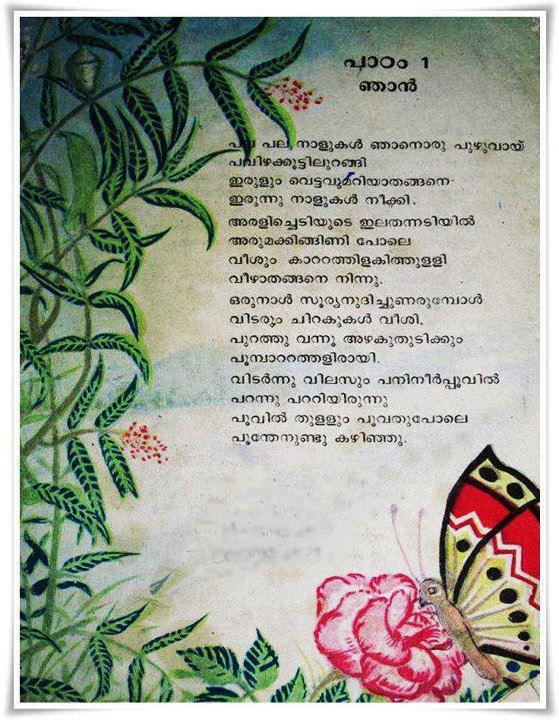
\includegraphics[width=\linewidth, height=8cm]{images/1988-reformed_text.jpg}
		\caption{Reformed Orthography in a Malayalam textbook -1988}
		\label{1988Text}
	\end{subfigure}
	\begin{subfigure}{.5\textwidth}
		\centering
		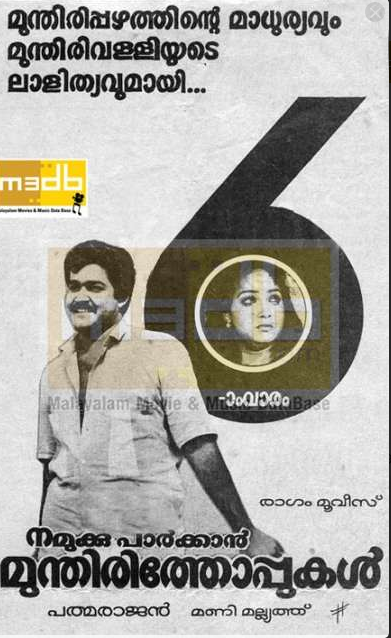
\includegraphics[width=\linewidth, height=8cm]{images/1986-Movieposter.png}
		\caption{A Malayalam movie poster from 1986 with everything written in traditional orthography.}
		\label{1986Movie}
	\end{subfigure}
	\caption{Co-existence of both orthographic styles in 1980s}
	\label{1986and1988}
\end{figure}

\section{Script in Digital Era}

\paragraph{}
The digitization of printing by early 1990s was yet another remarkable event. The pre-Unicode digital fonts in Malayalam were Malayalam letters mapped to the ASCII character space. Such fonts retained only a limited repertoire of conjuncts, because ASCII had the limitation of 256 codepoints. Also the signed notations of vowels and consonants were detached from the base grapheme. Digital fonts before the unicode era embraced the reformed orthography more closely. The publishing industry largely depended on these fonts for decades.

\paragraph{}
At the same time, writing Malayalam in non-digital, non-printing contexts continue to use traditional orthography. Wall paintings, artistic lettering used in magazines, movie titles continued using it as illustrated above

\paragraph{}
In 1998, an organization, named \textit{Rachana Aksharavedi} was formed to bring back the orthography with the help of technology advancement. At that time, Malayalam was not encoded in Unicode. Rachana Aksharavedi developed a font named \textit{Rachana} with about 1200 glyphs. Since there is no Unicode or opentype technology, it was a set of 6 fonts, each covering about 200 glyphs mapped to ASCII codepoints. A special editor known as Rachana Editor was required to automatically switch between these fonts and display Malayalam with data being English. This brave attempt was widely appreciated. A couple of years, in 2001 later Unicode encoding for Malayalam happened.

\subsection{Unicode and Advanced Digital Typography}

\paragraph{}
Unicode did not differentiate between the traditional and reformed orthography. Orthography was left to the the typogrphy/fonts layers. That means, the data remains same, the readers see that data using a font following traditional or reformed orthography as per their choice. This abstracted the reformation impact from data processing.

\paragraph{}
With the advent of Unicode based digital typography, complex conjunct formations and their rendering were no longer an impossibility. With only the basic graphemes encoded in Unicode, any long sequence of consonants and signs could be mapped to a single conjunct grapheme in signed or unsigned form. Complex rendering rules of the script can easily be handled by modern rendering engines. With these technical advancements, fonts which could very well support the traditional orthographic scheme of the Malayalam script emerged. 

\paragraph{}
The Rachana font was ported to Unicode. Parallel to that, more unicode fonts emerged, notably AnjaliOldLipi. In 2006, Swathanthra Malayalam Computing(SMC), a free software developer community became active in Malayalam computing. Along with various language processing tools and technology improvements, SMC released a dozen of Malayalam fonts. Except one, all followed traditional orthography and embrased the opentype technology. GNU/Linux systems came with these traditional orthography fonts by default. Schools and government institutions were using GNU/Linux systems because of Kerala government policy to use Free Software. The userbase of traditional orthography started to expand among digital Malayalam users. The IT education carriculum in schools also widely used these fonts.

\begin{figure}[H]
	\centering
	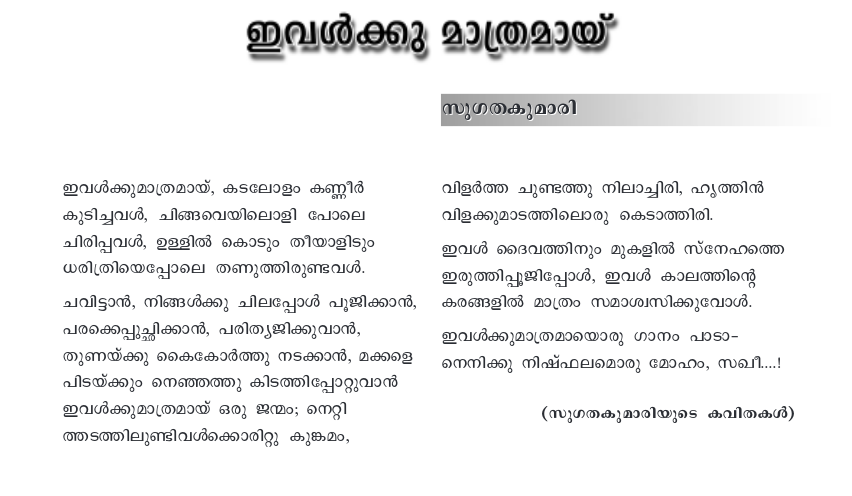
\includegraphics[scale=0.5]{images/2011-Malayalam-Textbook.png}
	\caption{Malayalam Textbook - 2011. ASCII based new orthography in print}
	\label{textbook2011}
\end{figure}

\paragraph{}
The typesetting tools and software adapted to ASCII based fonts were the default in the publishing industry since 1990s. Even after the encoding of Malayalam in Unicode in \textit{2001}, the printing and publishing industry continued their practices. The Figure \ref{textbook2011}, shows the usage of ASCII based reformed orthography in school textbooks printed in 2011. This was largely due to lack of unicode and complex script rendering support in major typesetting systems like Adobe Indesign. But these typsetting systems started supporting complex scripts and now we are seeing a highly accelerated adoption of Unicode and traditional orthography in printing.

\section{Contemporary Script Usage}
\paragraph{}
Now that the technology has matured enough to support the traditional orthography, it is becoming more and more popular. The traditional orthography fonts by SMC is widely used in web content. There are newspapers and portals that switched to traditional orthography. Popular illustrated weeklies and science magazines switched to traditional orthography style printing. 

\begin{figure}[H]
	\centering
	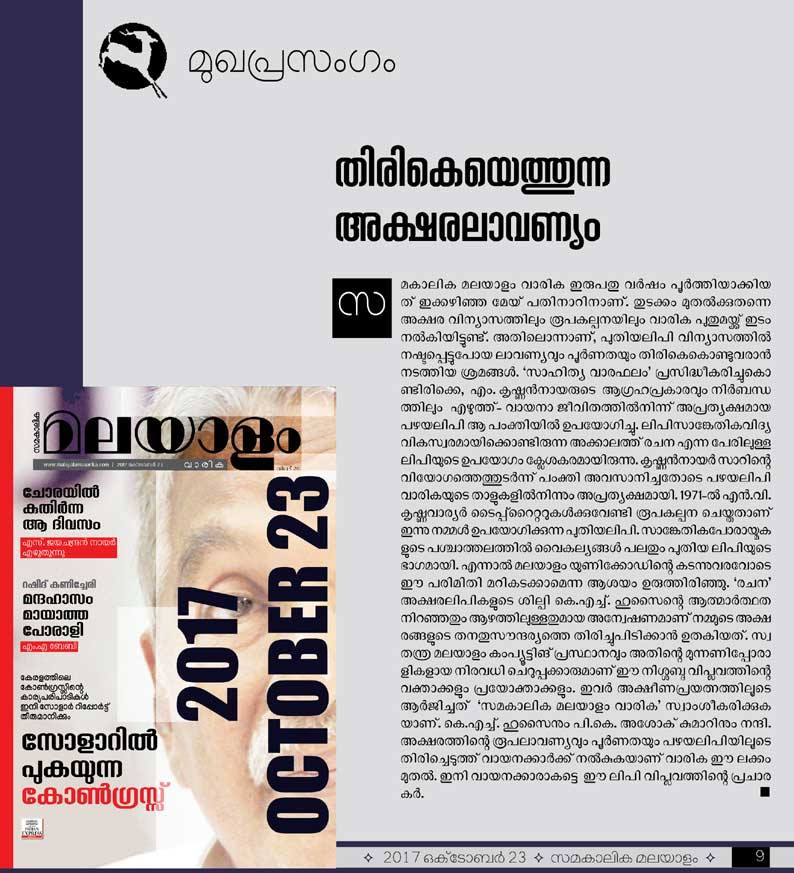
\includegraphics[scale=0.4]{images/samakalikamalayalam.jpg}
	\caption{Samakalika Malayalam, a popular illustrated weekly announcing their return to traditional orthography. 2017 October}
\end{figure}

\begin{figure}[H]
	\centering
	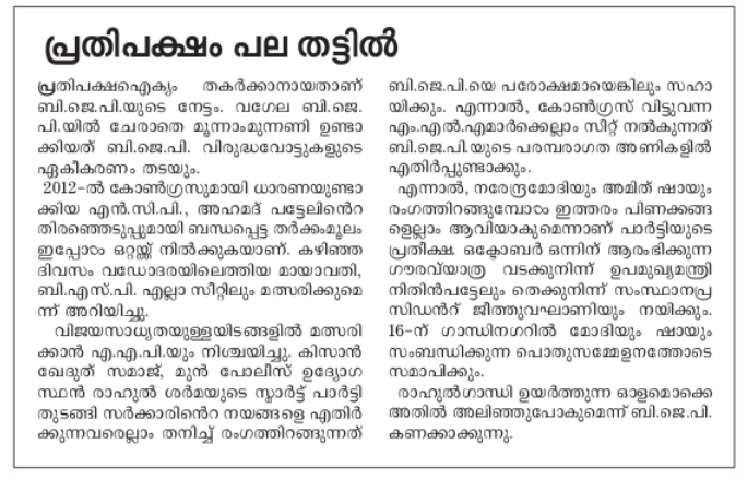
\includegraphics[scale=0.5]{images/2017-Mathrubhumi-newspaper.png}
	\caption{2017 Mathrubhumi news paper. Continues to follow semi-reformed orthography. But started using traditional orthography in supliments headlines.}
\end{figure}

\paragraph{}
Textbooks continue to follow reformed orthography. Children learn reformed orthography only in schools. But outside world is changing. 

\begin{figure}[H]
	\centering
	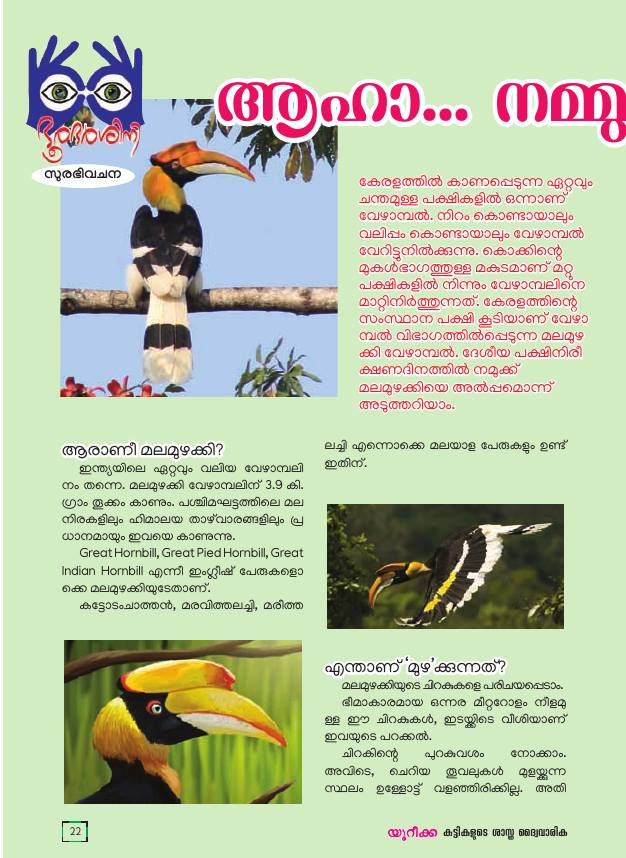
\includegraphics[scale=0.5]{images/2017-Eureka.jpg}
	\caption{Eureka, a famous science magazine for childrens changed to traditional orthography printing in November 2017.}
\end{figure}


\begin{figure}[H]
	\centering
	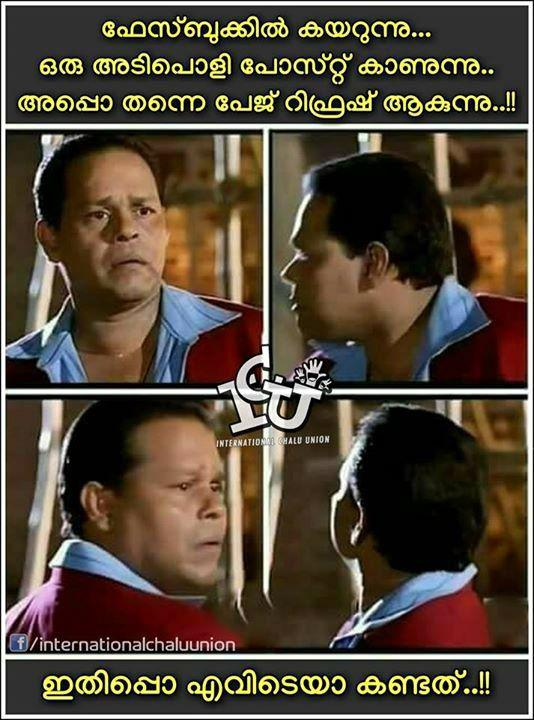
\includegraphics[width=0.7\textwidth, height=8cm]{images/2017-icu-meme.jpg}
	\caption{Internet meme example in Malayalam. Uses traditional orthography font. 2017 November}
\end{figure}


%\begin{figure}[h!]
%	\centering
%	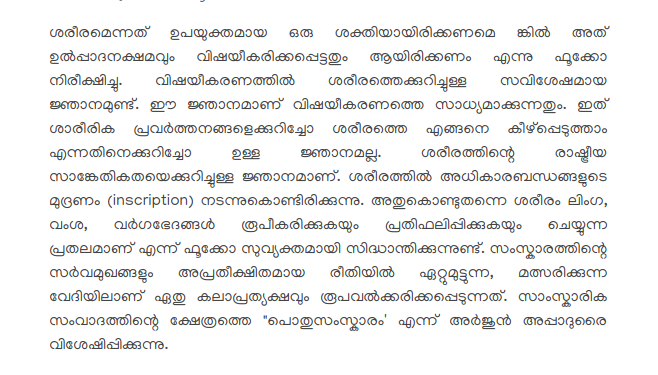
\includegraphics[width=1.0\textwidth]{images/Manjari-Body-Text.png}
%	\caption{2017 Manjari font- a widely used unicode font}
%\end{figure}


\paragraph{}
Kerala government is actively promoting unicode usage in the official documents. Government orders are now mostly in Meera font, a traditional orthography font by SMC. Identity cards used for voting and public distribution system (See figure \ref{rationcard}) etc also uses traditional orthography.

\begin{figure}[H]
 \centering
  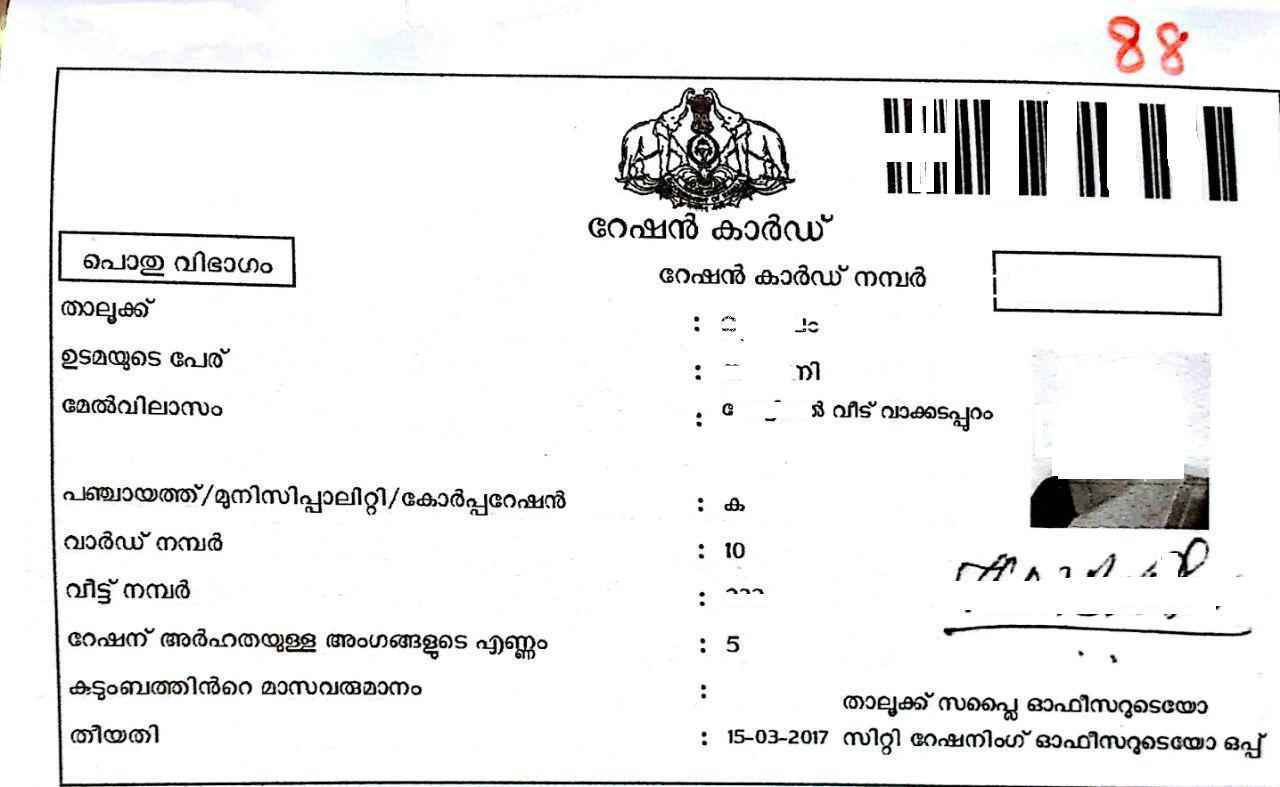
\includegraphics[width=1.0\textwidth,height=6cm ]{images/2017-rationcard.jpg}
   \caption{2017 Ration card}
  \label{rationcard}
\end{figure}


\begin{figure}[H]
 \centering
  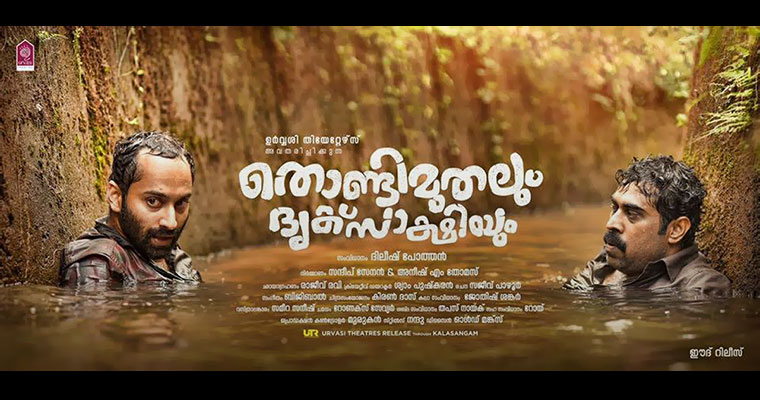
\includegraphics[width=1.0\textwidth]{images/2017-movieposter-Thondimuthal}
 \caption{A Malayalam movie poster from 2017. Uses mix of reformed and traditional orthogrophy for title.}
\end{figure}

\begin{figure}[H]
 \centering
  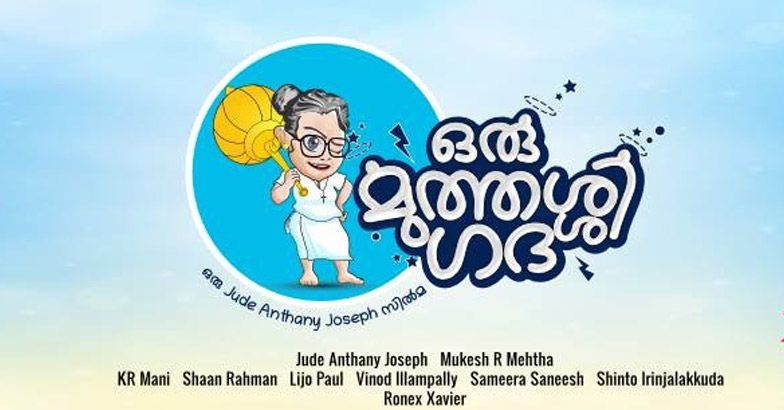
\includegraphics[width=1.0\textwidth]{images/2016-oru-muthashi-gadha}
 \caption{A Malayalam movie poster from 2016. Uses traditional orthogrophy for title.}
\end{figure}

\section{Conclusion}

\paragraph{}
Technology played a crucial role in defining the orthography of Malayalam from printing to digital age. When technology like typewriters had limitations script went through difficult reformation. But flourished again with the help digital technology. A single human generation is witnessing Malayalam's transition from traditional orthograhy to reformed orthography and then again to traditional orthography. 

\paragraph{}
Reformed orthography is sometimes referred as \textit{modern} and traditional as \textit{old}. But as traditional script is getting more popular in contemporary usage, calling it \textit{old} may not be right. So we conciously avoided those phrases in this paper.

\begin{thebibliography}{9}

\bibitem{babucherian} Babu Cheriyan, \textit{Bebjamin Bailiyum Malayala Sahithyavum} {\manjari{(ബെഞ്ചമിൻ ബെയിലിയും മലയാള സാഹിത്യവും}) }, Mahatma Gandhi University, Kottayam, 2008
\bibitem{gupthannair} S. Gupthan Nair, \textit{Gadyam Pinnitta Vazhikal}{\manjari{ (ഗദ്യം പിന്നിട്ട വഴികൾ)} }, DC Books, Kottayam
\bibitem{1971go} Order by the Government of Kerala, India, G. O. (P) 37/71/Edn. , \textit{Malayalam Script- Adoption of New Script for Use-Orders Issued}, Dated 23 March, 1971.
•


\end{thebibliography}

\end{document}
